\documentclass[10pt,twocolumn,letterpaper]{article}

\usepackage{cvpr}
\usepackage{times}
\usepackage{epsfig}
\usepackage{graphicx}
\usepackage{amsmath}
\usepackage{amssymb}
\usepackage{subfig}

% Include other packages here, before hyperref.

% If you comment hyperref and then uncomment it, you should delete
% egpaper.aux before re-running latex.  (Or just hit 'q' on the first latex
% run, let it finish, and you should be clear).
\usepackage[breaklinks=true,bookmarks=false]{hyperref}

\cvprfinalcopy % *** Uncomment this line for the final submission

\def\cvprPaperID{****} % *** Enter the CVPR Paper ID here
\def\httilde{\mbox{\tt\raisebox{-.5ex}{\symbol{126}}}}

% Pages are numbered in submission mode, and unnumbered in camera-ready
%\ifcvprfinal\pagestyle{empty}\fi
\setcounter{page}{1}
\begin{document}

%%%%%%%%% TITLE
\title{Image-Shape Matching with Shape Deformation}

\author{Tao Du\\
Stanford University\\
{\tt\small taodu@stanford.edu}
% For a paper whose authors are all at the same institution,
% omit the following lines up until the closing ``}''.
% Additional authors and addresses can be added with ``\and'',
% just like the second author.
% To save space, use either the email address or home page, not both
}

\maketitle
%\thispagestyle{empty}

%%%%%%%%% ABSTRACT
\begin{abstract}
\noindent
We present a global optimization approach to match keypoints from images and shapes while the shape can scale in three directions. The output of our method includes the camera matrix, the transform matrix between the world and the camera coordinates, and the scaling factor on the shape. We run our algorithm on three models with synthetic images. The experimental results show that our algorithm either manages to recover the ground truth values, or finds another physically plausible combination of parameters with small errors.
\end{abstract}

%%%%%%%%% BODY TEXT
\section{Introduction}

\noindent
Computer vision researchers have been working on 2D images for a long time, but recently 3D models become more and more prevalent in computer vision and computer graphics. As a result, we think it is of great significance to connect 3D shapes with large 2D image datasets. One of the most fundamental problems in this active area is to match image and shape together: assume we have a model $\mathbf{P}$, and we take a picture $\mathbf{I}$ of $\mathbf{P}$. If we are given a number of feature points in $\mathbf{P}$ and their corresponding positions in $\mathbf{I}$, can we estimate the camera matrix and the transformation so that we can project $\mathbf{P}$ into $\mathbf{I}$ to match all the key points correctly? It is well known that the matching between 2D pixels and 3D points can be solved by fitting a $3\times 4$ homography matrix, and the camera matrix $\mathbf{K}$ and the rotation matrix can extracted by RQ decomposition. Once $\mathbf{K}$ is defined, the translation vector $\mathbf{t}$ can be solved trivially as $\mathbf{K}$ is invertible, and solving $\mathbf{t}$ is as easy as solving an upper triangular linear system of equations.\\

\noindent
The solution described above works well theoretically, as long as the corresponding points are correctly labeled, and the shape in $\mathbf{I}$ and $\mathbf{P}$ are the same. However, we find this method fails some time in practice. The biggest issue is that one cannot expect a perfectly identical shape model is given for the image we are interested in matching. If we ignore the shape variation between the model we have and the model in the image, it turns out that the homography tends to absorb the variation into the camera matrix, and give a physically implausible camera model. As a simple example, let's consider stretching a cube in $x$-axis for 10 times. Instead of recognizing the scaling in $x$-axis, the algorithm will fit a perfect homography matrix, but with 10x focal length in $x$-axis for the camera! In some other examples, the homography matrix may contain badly skewed cameras, or camera model with largely deviated center points.\\

\noindent
As a result, we attempt to decompose the shape variation and the camera parameters in this project. We assume the shape is first scaled in three axes, then transformed into the camera space and projected into the image. Our goal is to estimate the scaling factor, the camera model, and the transformation at the same time. To achieve this, we use a different approach to extract the camera matrix from the homography, which enforces an ideal pinhole camera model with zero skew and the same focal lengths in $x$ and $y$ axes. We then propose a method to alternatively optimize the homography and the scaling factor until convergence.\\

\noindent
The remaining sections are organized as follows: Section 2 gives a short review of previous work; Section 3 covers the core of our optimization algorithm; The experimental results are provided in Section 4, and the final conclusion and discussions are given in Section 5.

%------------------------------------------------------------------------
\section{Related Work}
\noindent
\textbf{Intrinsic/extrinsic parameter estimation} Estimating the camera model and the extrinsic parameters have been heavily studied in camera calibration, single view metrology and structure from motion. Perhaps the most noticeable work is from Zhang ~\cite{zhang2000flexible}, who proposed a well-known method for camera model calibration using checkerboards. In this project we follow his method to decompose the intrinsic and extrinsic parameters from the homography.\\

\noindent
\textbf{Shape deformation} Summer \etal~\cite{sumner2007embedded} proposed an algorithm to manipulate the shape deformation based on graph nodes sampled from the shape. While their method is intuitive, they do not consider scaling the shape locally. Despite that, they provide a reasonable way to model the rigid local rotation and translation.\\

\noindent
Due to the time constraint, we only consider global scaling for the shapes in our project. Although this assumption greatly reduces the deformation space, we can still get valuable results which may help guide the follow up work in the future.

%------------------------------------------------------------------------
\section{Optimization Algorithm}

\noindent
In this section we describe our optimization algorithm in great details. The basic idea is to optimize the camera positions and the deformation functions alternatively. We have not yet proved the theoretical properties of the algorithms below, but we believe the root-mean-squared error decreases after each iteration, so the algorithm guarantees to converge into a local minima.

\subsection{Optimizing homography}

\noindent
Given $n$ pairs of correspondent points $\mathbf{p}_i\in\mathcal{R}^3$ and $\mathbf{q}_i\in\mathcal{R}^2$, $i=1,2,\cdots, n$, we want to fit $\mathbf{M}\in\mathcal{R}^{3\times 4}$ such that
\begin{equation}
\mathbf{q}_i=s_i\mathbf{M}\left[
\begin{array}{c}
\mathbf{p}_i\\
1
\end{array}
\right ]
\end{equation}
or equivalently
\begin{equation}
\begin{split}
&m_{11}p_{i1}+m_{12}p_{i2}+m_{13}p_{i3}+m_{14}\\
=&q_1(m_{31}p_{i1}+m_{32}p_{i2}+m_{33}p_{i3}+m_{34})\\
&m_{21}p_{i1}+m_{22}p_{i2}+m_{23}p_{i3}+m_{24}\\
=&q_2(m_{31}p_{i1}+m_{32}p_{i2}+m_{33}p_{i3}+m_{34})
\end{split}
\end{equation}
As a result, if we reshape $\mathbf{M}$ as a column vector $\mathbf{m}$, we can fit $\mathbf{m}$ by solving the following least square problem:
\begin{equation}
\begin{split}
\min_{\mathbf{m}}&\quad \|\mathbf{Am}\|_2^2\\
s.t.&\quad \|\mathbf{m}\|=1
\end{split}
\end{equation}
Here $\mathbf{A}\in\mathcal{R}^{2n\times 12}$. The optimal $\mathbf{m}$ can be found analytically by SVD.

\subsection{Optimizing intrinsic and extrinsic parameters}

\noindent
Once $\mathbf{M}$ is found, we will decompose $\mathbf{M}=\lambda\mathbf{K[R,t]}$. Here we borrow the idea from Zhang~\cite{zhang2000flexible} to fit both the camera matrix $\mathbf{K}$, the rotation matrix $\mathbf{R}$ and the translation vector $\mathbf{t}$. We use $\mathbf{m}_i$ to represent the $i$-th column in $\mathbf{M}$.\\

\noindent
The camera matrix $\mathbf{K}$ is an upper triangular matrix:
\begin{equation}
\mathbf{K}=\left [
\begin{array}{ccc}
f & 0 & x \\
0 & f & y \\
0 & 0 & 1
\end{array}
\right ]
\end{equation}
Note that we assume the camera does not have any distortion, and the aspect ratio is 1. Both assumptions are reasonable: if we allow $\mathbf{K}_{12}\neq 0$, or if we allow $\mathbf{K}_{11}\neq\mathbf{K}_{12}$, they will absorb the effects of rotation and scaling, which should actually be explained by the shape deformation. Once $\mathbf{K}$ is determined, $\mathbf{t}$ can be easily solved by $\mathbf{t} = \mathbf{K}^{-1}\mathbf{m}_4$. So the main challenge is to solve $\mathbf{K}$ and $\mathbf{R}$. If we use $\mathbf{r}_i$ to denote the $i$-th column in $\mathbf{R}$, we will have:
\begin{equation}
\begin{split}
\lambda\mathbf{K}\mathbf{r}_1=&\mathbf{m}_1\\
\lambda\mathbf{K}\mathbf{r}_2=&\mathbf{m}_2\\
\lambda\mathbf{K}\mathbf{r}_3=&\mathbf{m}_3\\
\mathbf{r}_1=&\lambda^{-1}\mathbf{K}^{-1}\mathbf{m}_1\\
\mathbf{r}_2=&\lambda^{-1}\mathbf{K}^{-1}\mathbf{m}_2\\
\mathbf{r}_3=&\lambda^{-1}\mathbf{K}^{-1}\mathbf{m}_3\\
\end{split}
\end{equation}
For any $i\neq j$, we have the constraint $\mathbf{r}_i^\top\mathbf{r}_j=0$:
\begin{equation}
\begin{split}
\mathbf{m}_1^\top\mathbf{K}^{-\top}\mathbf{K}^{-1}\mathbf{m}_2&=0\\
\mathbf{m}_1^\top\mathbf{K}^{-\top}\mathbf{K}^{-1}\mathbf{m}_3&=0\\
\mathbf{m}_2^\top\mathbf{K}^{-\top}\mathbf{K}^{-1}\mathbf{m}_3&=0\\
\end{split}
\end{equation}
Moreover, $\mathbf{r}_i$ has the same length:
\begin{equation}
\begin{split}
\mathbf{m}_1^\top\mathbf{K}^{-\top}\mathbf{K}^{-1}\mathbf{m}_1&=\mathbf{m}_2^\top\mathbf{K}^{-\top}\mathbf{K}^{-1}\mathbf{m}_2\\
\mathbf{m}_2^\top\mathbf{K}^{-\top}\mathbf{K}^{-1}\mathbf{m}_2&=\mathbf{m}_3^\top\mathbf{K}^{-\top}\mathbf{K}^{-1}\mathbf{m}_3\\
\end{split}
\end{equation}
All the constraints contain $\mathbf{K}^{-\top}\mathbf{K}^{-1}$. Note that $\mathbf{K}^{-1}$ is
\begin{equation}
\mathbf{K}^{-1}=\left [
\begin{array}{ccc}
\frac{1}{f} & 0 & -\frac{x}{f} \\
0 & \frac{1}{f} & -\frac{y}{f} \\
0 & 0 & 1
\end{array}
\right ]
\end{equation}
So we can define
\begin{equation}
\begin{split}
\mathbf{B}=&\mathbf{K}^{-\top}\mathbf{K}^{-1}\\
=&\left [
\begin{array}{ccc}
\frac{1}{f} & 0 & 0 \\
0 & \frac{1}{f} & 0 \\
-\frac{x}{f} & -\frac{y}{f} & 1
\end{array}
\right ]
\left [
\begin{array}{ccc}
\frac{1}{f} & 0 & -\frac{x}{f} \\
0 & \frac{1}{f} & -\frac{y}{f} \\
0 & 0 & 1
\end{array}
\right ]\\
=&\left [
\begin{array}{ccc}
\frac{1}{f^2} & 0 & -\frac{x}{f^2} \\
0 & \frac{1}{f^2} & -\frac{y}{f^2} \\
-\frac{x}{f^2} & -\frac{y}{f^2} & \frac{x^2+y^2}{f^2} + 1
\end{array}
\right ]\\
=&\left [
\begin{array}{ccc}
B_{11} & 0 & B_{13} \\
0 & B_{11} & B_{23} \\
B_{13} & B_{23} & B_{33}
\end{array}
\right ]
\end{split}
\end{equation}
Since $B$ is symmetric, it only contains $4$ variables. Now for any $i$ and $j$, we can rewrite the constraints as:
\begin{equation}
\begin{split}
\mathbf{m}_i^\top\mathbf{B}\mathbf{m}_j=&\mathbf{v}_{ij}^\top\mathbf{b}\\
=&\left [
\begin{array}{c}
m_{i1}m_{j1}+m_{i2}m_{j2}\\
m_{i1}m_{j3}+m_{i3}m_{j1}\\
m_{i2}m_{j3}+m_{i3}m_{j2}\\
m_{i3}m_{j3}
\end{array}
\right ]^\top
\left [
\begin{array}{c}
B_{11} \\
B_{13} \\
B_{23} \\
B_{33}
\end{array}
\right ]\\
\end{split}
\end{equation}
Putting them together yields the following results:
\begin{equation}
\mathbf{Vb}=\left [
\begin{array}{c}
\mathbf{v}_{12}^\top\\
\mathbf{v}_{13}^\top\\
\mathbf{v}_{23}^\top\\
(\mathbf{v}_{11}-\mathbf{v}_{22})^\top\\
(\mathbf{v}_{22}-\mathbf{v}_{33})^\top\\
\end{array}
\right ]\mathbf{b}=0
\end{equation}
As a result, we can solve the following optimization problem to get $\mathbf{B}$:
\begin{equation}
\begin{split}
\min_{\mathbf{b}}&\quad \|\mathbf{Vb}\|_2^2\\
s.t.&\quad \|\mathbf{b}\|=1
\end{split}
\end{equation}
which again can be solved by SVD. One caveat in this optimization is that the optimal $\mathbf{b}$ need to be converted into $\mathbf{B}$ up to scale:
\begin{equation}
\begin{split}
&\beta\mathbf{B}\\
=&\left [
\begin{array}{ccc}
b_1 & 0 & b_2 \\
0 & b_1 & b_3 \\
b_2 & b_3 & b_4
\end{array}
\right ]\\
=&\left [
\begin{array}{ccc}
\frac{\beta}{f^2} & 0 & -\frac{\beta x}{f^2} \\
0 & \frac{\beta}{f^2} & -\frac{\beta y}{f^2} \\
-\frac{\beta x}{f^2} & -\frac{\beta y}{f^2} & \beta\frac{x^2+y^2}{f^2} + \beta
\end{array}
\right ]\\
\end{split}
\end{equation}
The camera parameters then can be pulled directly from $\mathbf{b}$:
\begin{equation}
\begin{split}
x=&-\frac{b_2}{b_1}\\
y=&-\frac{b_3}{b_1}\\
\beta=&b_4-\frac{b_2^2+b_3^2}{b_1}\\
f=&\sqrt{\frac{\beta}{b_1}}=\frac{\sqrt{b_4b_1-(b_2^2+b_3^2)}}{|b_1|}
\end{split}
\end{equation}
Once $\mathbf{K}$ is known, $\mathbf{R}$ can be solved by computing $\mathbf{R}\propto\mathbf{K}^{-1}[\mathbf{m}_1,\mathbf{m}_2,\mathbf{m}_3]$, and using SVD to make sure $\mathbf{R}$ is orthogonal.

\subsection{Optimizing shape deformation}

\noindent
Here we only consider scaling the shape in its principal axis. Specifically, we want to estimate a diagonal matrix $\mathbf{S}$:
\begin{equation}
\mathbf{S}=\left [
\begin{array}{ccc}
s_x & 0 & 0 \\
0 & s_y & 0 \\
0 & 0 & s_z
\end{array}
\right ]
\end{equation}
For each pair of correspondent points $\mathbf{p}_i$ and $\mathbf{q}_i$, we want to fit $\mathbf{S}$ such that:
\begin{equation}
\begin{split}
\mathbf{q}_i=&s_i\mathbf{K}(\mathbf{R}\mathbf{S}\mathbf{p}_i + \mathbf{t})\\
=&s_i\mathbf{K}(\mathbf{R}\mathbf{P}_i\left [
\begin{array}{c}
s_x \\
s_y \\
s_z
\end{array}
\right ] + \mathbf{t})
\end{split}
\end{equation}
Here $\mathbf{P}_i$ is a diagonal matrix:
\begin{equation}
\mathbf{P}_i=\left [
\begin{array}{ccc}
p_{i1} & 0 & 0\\
0 & p_{i2} & 0\\
0 & 0 & p_{i3}
\end{array}
\right ]
\end{equation}
Define $\mathbf{D}^i = \mathbf{KRP}_i\in\mathcal{R}^{3\times 3}$ and $\mathbf{o}=\mathbf{Kt}\in\mathcal{R}^{3}$, we get 2 linear equations for each pair of correspondence:
\begin{equation}
\begin{split}
&d^i_{11}s_x+d^i_{12}s_y+d^i_{13}s_z+o_1\\
=&q_{i1}(d^i_{31}s_x+d^i_{32}s_y+d^i_{33}s_z+o_3)\\
&d^i_{21}s_x+d^i_{22}s_y+d^i_{23}s_z+o_2\\
=&q_{i2}(d^i_{31}s_x+d^i_{32}s_y+d^i_{33}s_z+o_3)\\
\end{split}
\end{equation}
which can be formulated into a linear least square problem:
\begin{equation}
\begin{split}
\min_{\mathbf{s}\in\mathcal{R}^3}&\quad \|\mathbf{D}\mathbf{s}-\mathbf{O}\|_2^2
\end{split}
\end{equation}
Here $\mathbf{D}\in\mathcal{R}^{2n\times 3}$, $\mathbf{O}\in\mathcal{R}^{2n}$, and $\mathbf{s}=(\mathbf{D}^\top\mathbf{D})^{-1}\mathbf{D}^\top\mathbf{O}$.

\subsection{Putting it together}

\noindent
Once we figure out how to optimize camera parameters and scaling parameters, we loop over these variables and optimize them alternatively. In each iteration, we start from fitting the homography and extract the camera intrinsic parameter $\mathbf{K}$, rotation matrix $\mathbf{R}$ and translation vector $\mathbf{t}$, then we fix $\mathbf{K}$, $\mathbf{R}$, $\mathbf{t}$, optimize the scaling factor $\mathbf{s}$, and scaling $\mathbf{p}_i$ by $\mathbf{s}$. We use the scaled $\mathbf{p}_i$ in the next iteration. We terminate the optimization as long as $\mathbf{s}$ converges to $[1,1,1]^\top$.

%------------------------------------------------------------------------
\section{Experiments}

\begin{table*}
\begin{center}
\begin{tabular}{|l|c|c|c|c|c|c|}
\hline
Model & rel($\mathbf{K}$) & rel($\mathbf{R}$) & $\|\mathbf{t}_g\|/\|\mathbf{t}_e\|$ & $\|\mathbf{s}_g\|/\|\mathbf{s}_e\|$ & rel($\hat{\mathbf{t}}$) & rel($\hat{\mathbf{s}}$) \\
\hline\hline
Chair & 1.1465e-05 & 7.2471e-06 & 0.8248 & 0.8248 & 1.4494e-05 & 8.4682e-06 \\
Bunny & 0.1803 & 0.1309 & 1.3409 & 1.2367 & 0.2809 & 0.1260 \\
Dragon & 3.7028e-06 & 2.9360e-06 & 0.9905 & 0.9905 & 5.8720e-06 & 1.7058e-06 \\
\hline
\end{tabular}
\end{center}
\caption{Quantitative analysis for all the models. The bunny model has large relative error because we find a different combination of scaling and camera parameters which yield small rms error.}
\label{tb:err}
\end{table*}

\begin{figure}
\begin{center}
	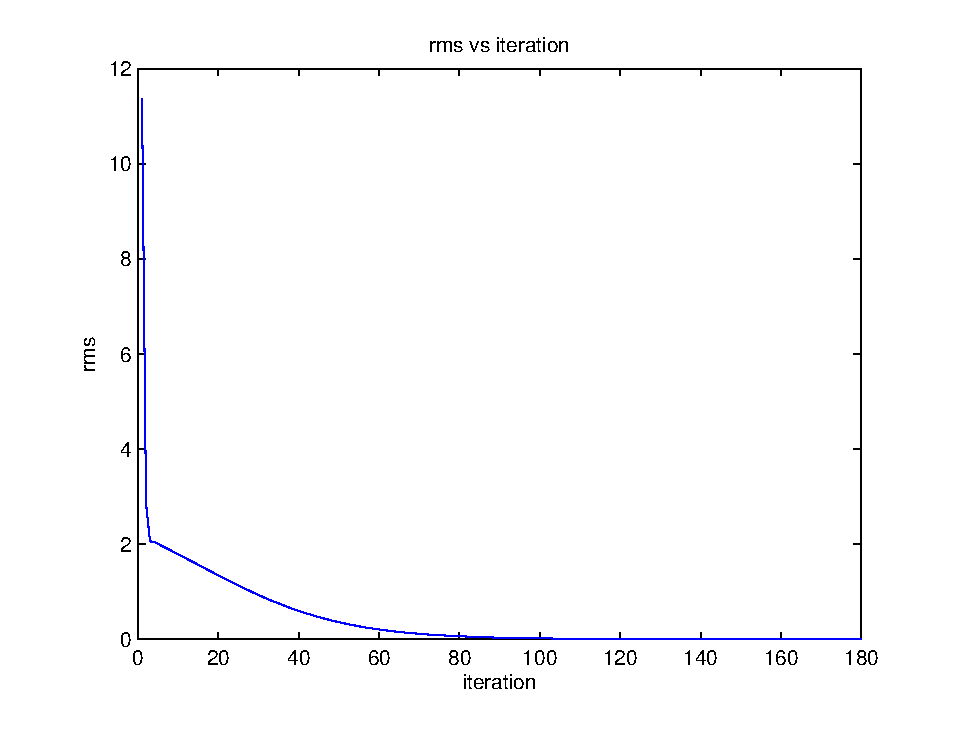
\includegraphics[scale=0.5]{chair-figure.eps}
\end{center}
	\caption{The rms error for Chair. The horizontal axis: the number of iterations; The vertical axis: the rms error in pixel.}
\label{fig:chairplot}
\end{figure}

\noindent
In this section we test our algorithms with three models: Chair from ShapeNet~\cite{shapenet2015}, Bunny and Dragon from the Stanford 3D Scanning Repository~\cite{stanford3d2014}. For all the experiments below, we first scale the model by a predefined scaling factor $\mathbf{s}$, then we use PBRT~\cite{pharr2010pbrt} to render a synthetic image. $\mathbf{p}_i$ are all the vertices in the shape, and $\mathbf{q}_i$ are the projected pixel positions of $\mathbf{p}_i$ in the synthetic image. We recover the camera position and the scaling factor, and compare them with the ground truth values.\\

\noindent
To quantitatively evaluate the results, we provide the relative error between the ground truth $\mathbf{K}_g$, $\mathbf{R}_g$, and the corresponding estimation $\mathbf{K}_e$, $\mathbf{R}_e$:
\begin{equation}
\begin{split}
\textrm{rel}(\mathbf{X})=&\frac{\|\mathbf{X}_g-\mathbf{X}_e\|}{\|\mathbf{X}_g\|}
\end{split}
\end{equation}
We use Frobenius norm for matrices and 2-norm for vectors.\\

\noindent
Note that $\mathbf{t}$ and $\mathbf{s}$ are up to scale simultaneously: if $\mathbf{q}_i=s_i\mathbf{K}(\mathbf{R}\mathbf{S}\mathbf{p}_i + \mathbf{t})$ holds, so does $\mathbf{q}_i=(s_i/\lambda)\mathbf{K}(\mathbf{R}\lambda\mathbf{S}\mathbf{p}_i + \lambda\mathbf{t})$. As a result, for $\mathbf{t}$ and $\mathbf{s}$ we expect the ground truth and the estimated vectors are parallel, and the ratio between their lengths are the same:
\begin{equation}
\begin{split}
\frac{\|\mathbf{t}_g\|}{\|\mathbf{t}_e\|}=&\frac{\|\mathbf{s}_g\|}{\|\mathbf{s}_e\|}\\
\hat{\mathbf{t}}_g=&\hat{\mathbf{t}}_e\\
\hat{\mathbf{s}}_g=&\hat{\mathbf{s}}_e\\
\end{split}
\end{equation}
Here $\hat{\mathbf{x}}=\mathbf{x}/\|\mathbf{x}\|$, or the unit vector in its direction.\\

\noindent
As we use an iterative algorithm, we also compute the rms error in each iteration. The rms error is defined as the root-mean-squared value of the difference between the projected pixel position of the shape vertex, and its corresponding pixel in the synthetic image.\\

\noindent
To evaluate the results qualitatively, we also blend the projection of the model and the synthetic image in a single image. The overlap of the two contours indicates the better matching results.\\

\begin{figure*}
\begin{center}
	\includegraphics[scale=0.4]{image-shape.eps}
\end{center}
   \caption{The synthetic image and the original models used in the experiments. Top: synthetic images for scaled chair, bunny and dragon model; Bottom: the original chair, bunny and dragon model.}
\label{fig:imageshape}
\end{figure*}

\noindent
\textbf{Chair} The synthetic image for the scaled chair model and the original chair is displayed in Figure ~\ref{fig:imageshape}. We set $\mathbf{s}_g=[0.6, 0.8, 1.2]^\top$ in this example. The algorithm terminates in 180 iterations. The rms error in each iteration is plotted in Figure ~\ref{fig:chairplot}. The rms error decreases quickly at the beginning, then it refines the camera parameters and the scaling factor, as shown in the long tail of the plot.\\

\noindent
Figure ~\ref{fig:chairgrid} shows the overlap between optimized chair models and the original synthetic image in 8 different iterations. Iteration 0 quickly aligns the unscaled model with the scaled one in the image, which turns out to be a good guess for optimizing the scale factor in the next few iterations. Within 5 iterations the algorithm already aligns the scaled model and the synthetic image perfectly. The quantitative errors between each pairs of parameters are listed in Table ~\ref{tb:err}.

\begin{figure}[t]
\begin{center}
	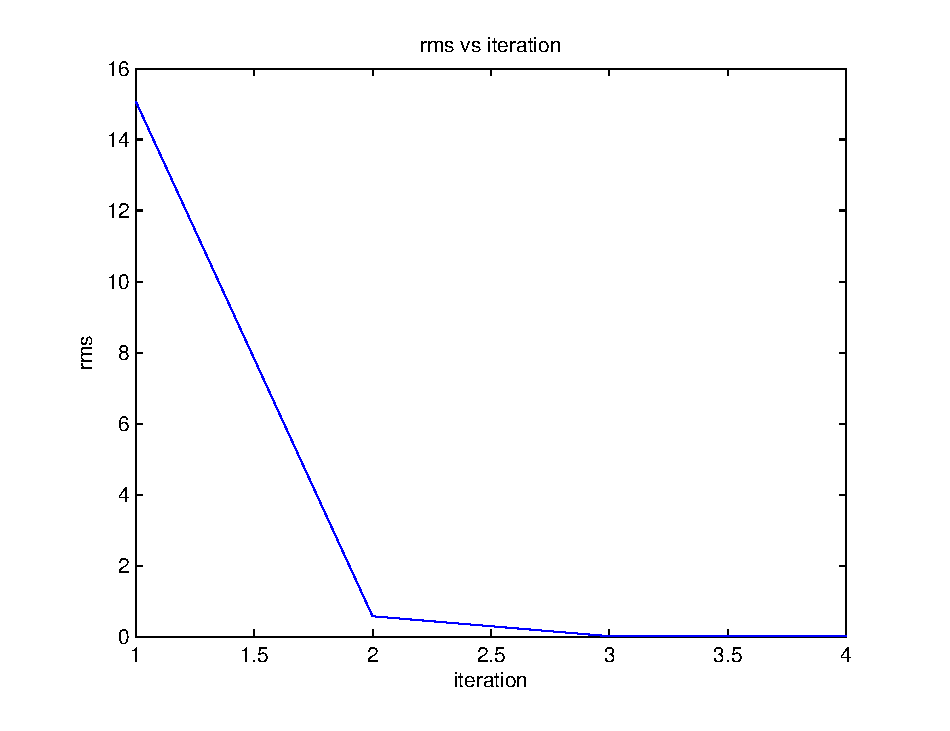
\includegraphics[scale=0.5]{bunny-figure.eps}
\end{center}
	\caption{The rms error for Bunny. The horizontal axis: the number of iterations; The vertical axis: the rms error in pixel.}
\label{fig:bunnyplot}
\end{figure}

\begin{figure*}
\begin{center}
	\includegraphics[scale=0.4]{chair-grid.eps}
\end{center}
   \caption{Blending the optimized chair model and the synthetic image in 8 iterations. Top row: iteration 0, 1, 2, 5; Bottom row: iteration 10, 50, 150, 180.}
\label{fig:chairgrid}
\end{figure*}

\begin{figure}[b]
\begin{center}
	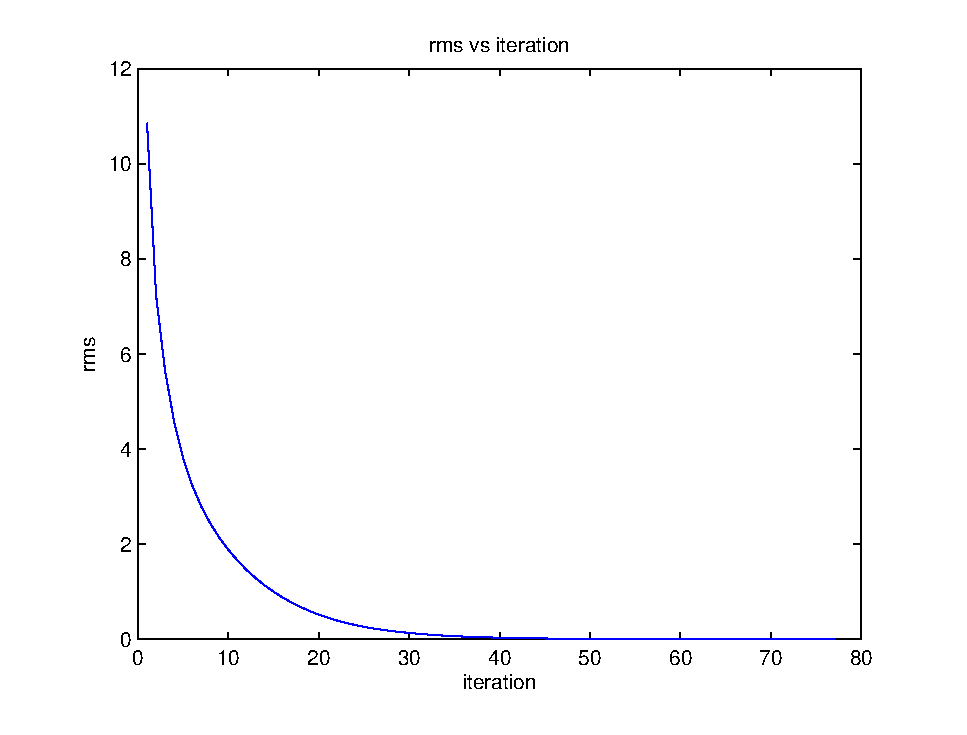
\includegraphics[scale=0.5]{dragon-figure.eps}
\end{center}
	\caption{The rms error for Dragon. The horizontal axis: the number of iterations; The vertical axis: the rms error in pixel.}
\label{fig:dragonplot}
\end{figure}

\noindent
\textbf{Bunny} The synthetic image and the original bunny is displayed in Figure ~\ref{fig:imageshape}. We set $\mathbf{s}_g=[1.25, 0.8, 1.1]^\top$ in this example. It takes only 4 iterations for the algorithm to converge. The rms error in each iteration is plotted in Figure ~\ref{fig:bunnyplot}.\\

\noindent
One notable difference between Bunny and Chair is that Bunny does not converge to the ground truth parameters. Nevertheless, we manage to find another combination of scaling factor and camera parameters that works well for matching the images and the bunny. This phenomenon again indicates that our image-shape matching problem is under-determinant.

\begin{figure*}[t]
\begin{center}
	\includegraphics[scale=0.4]{bunny-grid.eps}
\end{center}
   \caption{Blending the optimized chair model and the synthetic image in iteration 0, 1, 2, 4.}
\label{fig:bunnygrid}
\end{figure*}

\begin{figure*}[t]
\begin{center}
	\includegraphics[scale=0.4]{dragon-grid.eps}
\end{center}
   \caption{Blending the optimized dragon model and the synthetic image in 8 iterations. Top row: iteration 0, 1, 2, 5; Bottom row: iteration 10, 25, 50, 78.}
\label{fig:dragongrid}
\end{figure*}

\noindent
\textbf{Dragon} Figure ~\ref{fig:imageshape} displays the synthetic dragon image and the orginal dragon model. We set $\mathbf{s}_g=[1.3, 0.7, 0.9]^\top$ in this example. The algorithm terminates in 78 iterations. The rms error in each iteration is plotted in Figure ~\ref{fig:dragonplot}. As in the previous examples we present the overlap between models and images in Figure ~\ref{fig:dragongrid}. Unlike the Chair and Bunny example, it takes much more iterations to register the model with the image. This is as expected since the dragon contains much more fine-grained details.

%------------------------------------------------------------------------
\section{Conclusion}

\noindent
In this project we present a global optimization method for image and shape mapping with shape deformations. We assume the correspondent points between image and shape are given, and the shape scales in its 3 principal axes. We alternatively optimize the camera parameters and the scaling parameters. Our experiments demonstrate that given accurate correspondent points, this global optimization approach works well in finding good parameters to achieve small error.\\

\noindent
This work can be improved in the following ways: One interesting extension is to implement a non-trivial shape deformation model, especially for models that allow local deformation in multiple parts of shapes. This kind of shape variation is prevalent in man-made objects. Moreover, our work can be integrated with correspondence detection approaches to build a completely automatic pipeline.

{\small
\bibliographystyle{ieee}
\bibliography{reportbib}
}

\end{document}
